\documentclass{article}
\usepackage{geometry,tikz}
\usetikzlibrary{calc,fit,arrows,positioning,shapes,shadows}
\geometry{paperwidth=20cm, paperheight=8cm,left=2pt,right=2pt,top=2pt,bottom=2pt}
\pagestyle{empty}
\setlength{\parindent}{0pt}
\tikzset{%
ref/.style={rounded corners=5mm,red,-stealth},
der/.style={rounded corners,black,stealth-,densely dotted},
cont/.style={rounded corners,-stealth},
uses/.style={rounded corners,)-},
templ/.style={rounded corners,blue,-stealth},
point/.style={rounded corners,violet,-stealth,double},
subpartA/.style={draw,dashed,rounded corners=20pt,very thick},
partA/.style={draw,draw opacity=#1,dashed,rounded corners=20pt,very thick,fill = white, drop shadow={shadow xshift = 5mm, shadow yshift = -5mm, opacity=#1}},
no/.style={opacity=0.2,text opacity=0.2},
partA/.default=1
}
\pgfdeclarelayer{background}
\pgfdeclarelayer{behind}
\pgfsetlayers{behind,background,main}
\newcommand{\obj}[2][\relax]{\ifx#1\relax\texttt{#2<CoeffType>}\else\texttt{#1<CoeffType,#1>}\fi}
\newcommand{\buildboundingbox}[4]{%
\useasboundingbox ([yshift=10pt]#1.north) -| ([xshift=8pt]#2.east) |- ([yshift=-10pt]#3.south) -| ([xshift=-8pt]#4.west) |- ([yshift=10pt]#1.north)
}
\begin{document}
\centering
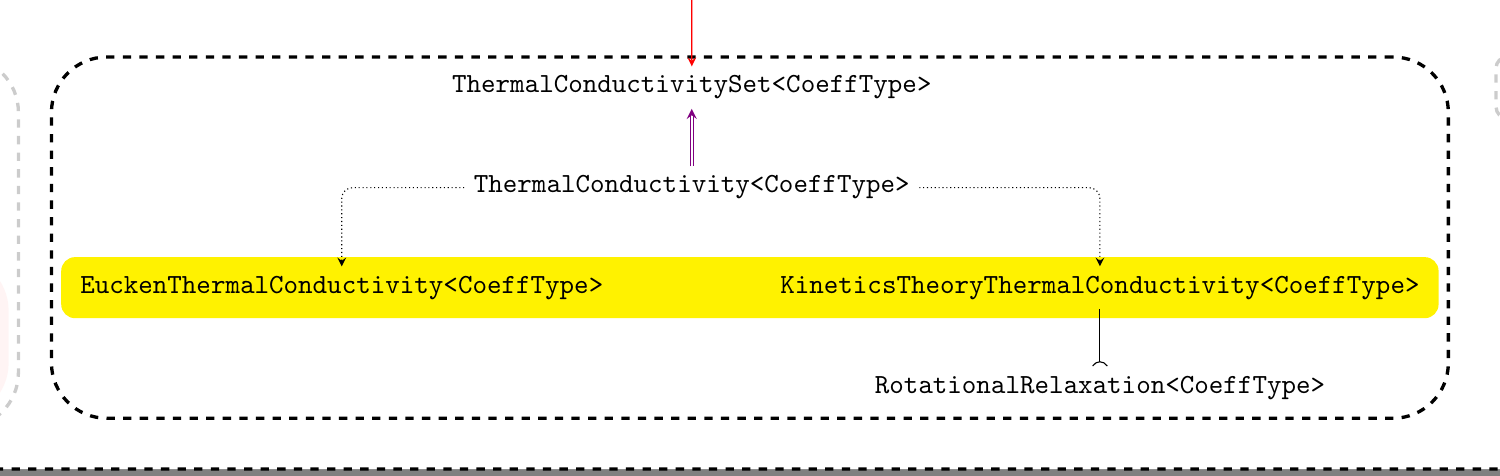
\begin{tikzpicture}[x=6cm,y=1cm,
                    every node/.append style={baseline}]
%%%%%%%%%%%%%%%%%%%%%%%%%
%%% all around core
%%%%%%%%%%%%%%%%%%%%%%%%%
%\node (SpecEnum) at (-7.5,1)  {\texttt{SpeciesEnum}};
%%
%% Core
\begin{scope}[every node/.append style={no},every path/.append style={no}]
\node (LenJon)   at (-6,-11) {\obj{LennardJonesPotential}};
\node (TranSpec) at (-6,-10) {\obj{TransportSpecies}};
\node (TranMix)  at (-6,-8)  {\obj{TransportMixture}};
\node (ChemSpec) at (-5,-9)  {\obj{ChemicalSpecies}};
\node (ChemMix)  at (-5,-8)  {\obj{ChemicalMixture}};
\draw[ref]   (ChemSpec) -- (ChemMix);
\draw[cont]  (LenJon)   -- (TranSpec);
\draw[point] (TranSpec) -- ([yshift=-15pt]TranMix);
\draw[ref]   (ChemMix)  -- ([yshift=15pt]TranMix);
\begin{pgfonlayer}{background}
\node[fit = (ChemSpec) (ChemMix) (LenJon) (TranSpec) (TranMix), rounded corners=20pt, fill = teal!20, shape = ellipse] (core) {};
\end{pgfonlayer}
%%
%%%%%
%%% transport
%%%%
\node[below = 2cm] (WilEval)  at (core.south) {\obj{WilkeEvaluator}};
\node[below = 1cm] (WilMix)   at (WilEval)    {\obj{WilkeMixture}};
\node[below = 1cm] (PureSpec) at (WilMix)     {\obj{PureSpeciesMixture}};
\draw[ref] (PureSpec) -- (WilMix);
\draw[ref] (WilMix)   -- (WilEval);
%%% diffusion
\node[below left = 2cm and 10cm] (DiffSet)    at (PureSpec) {\obj{DiffusionSet}};
\node[below = 1cm]              (BinMolDiff) at (DiffSet)         {\obj{MolecularBinaryDiffusion}};
\draw[cont]  (BinMolDiff) -- (DiffSet);
\begin{pgfonlayer}{background}
\node[fit = (DiffSet) (BinMolDiff), subpartA] (diffusion) {};
\end{pgfonlayer}
%%
%%% viscosity
\node[below left = 2cm and -5mm] (VisSet)  at (PureSpec) {\obj{ViscositySet}};
\node[below = 1cm] (Visco)   at (VisSet)     {\obj{Viscosity}};
\node[below = 2cm] (KinTVis) at (Visco.south) {\obj{KineticsTheoryViscosity}};
\node[below left  = 1cm] (SuthVis) at (Visco.south) {\obj{SutherlandViscosity}};
\node[below right = 1cm] (BlotVis) at (Visco.south) {\obj{BlottnerViscosity}};
\draw[point] (Visco)   -- (VisSet);
\draw[der]   (BlotVis) |- (Visco);
\draw[der]   (SuthVis) |- (Visco);
\draw[der]   (KinTVis) -- (Visco);
\begin{pgfonlayer}{background}
% viscosity model
\node[fit = (KinTVis) (SuthVis) (BlotVis), rounded corners=20pt, fill = red!20] (viscosityMod) {};
% viscosity
\node[fit = (viscosityMod) (VisSet), subpartA] (visco) {};
\end{pgfonlayer}
\end{scope}
%%
%% thermal conduction
\node[below right = 2cm and 10cm] (TauSet)   at (PureSpec) {\obj{ThermalConductivitySet}};
\node[below = 1cm]               (Tau)      at (TauSet)          {\obj{ThermalConductivity}};
\node[below right = 1cm and 1cm] (KinTTau)  at (Tau)             {\obj{KineticsTheoryThermalConductivity}};
\node[below left  = 1cm and 1cm] (EuckTau)  at (Tau)             {\obj{EuckenThermalConductivity}};
\node[below = 1cm]               (RotRelax) at (KinTTau)         {\obj{RotationalRelaxation}};
\draw[point] (Tau)      -- (TauSet);
\draw[der]   (KinTTau)  |- (Tau);
\draw[der]   (EuckTau)  |- (Tau);
\draw[uses]  (RotRelax) -- (KinTTau);
\begin{pgfonlayer}{background}
% therm cond models
\node[fit = (KinTTau) (EuckTau), rounded corners = 5pt, fill = yellow] (thermalCondMod) {};
% therm cond
\node[fit = (thermalCondMod) (TauSet) (RotRelax), subpartA] (thermalCond) {};
\end{pgfonlayer}
\begin{scope}[every node/.append style={no},every path/.append style={no}]
%% lewis diffusivity
\node[below right = 2cm and 23.5cm]  (LewisDiff)  at (PureSpec) {\obj{ConstantLewisDiffusivity}};
\begin{pgfonlayer}{background}
\node[fit = (LewisDiff), subpartA, rounded corners] (diffusivity) {};
\end{pgfonlayer}
\draw[ref] (DiffSet) |- (PureSpec);
\draw[ref,rounded corners=10pt] (VisSet)  |- ($(VisSet.north)!0.5!(PureSpec.south)$) -|(PureSpec);
\draw[ref] (TauSet)  |- (PureSpec);
%%
%% thermo
\node[above left = 2mm and 4cm] (CEAthermo) at (core.north west) {\obj{CEAThermodynamics}};
\node[above = 1cm]              (CEAcurve)  at (CEAthermo.north) {\obj{CEACurveFit}};
\draw[point] (CEAcurve) -- (CEAthermo);
%%
%% Kinetics
\node[above = 1cm] (kinEval)     at (core.north)        {\obj{KineticsEvaluator}};
\node[above = 5mm] (reactionSet) at (kinEval.north)     {\obj{ReactionSet}};
\node[above = 5mm] (reaction)    at (reactionSet.north) {\obj{Reaction}};
%% chem process
\node[above right = 2.0cm and 0.2cm] (TB)   at (reaction.north)              {\obj{ThreeBodyReaction}};
\node[right = 1cm]                   (Dupl) at (TB.east)                     {\obj{DuplicateReaction}};
\node[above = 1cm]                   (Elem) at ($(TB.east)!0.5!(Dupl.west)$) {\obj{ElementaryReaction}};
\node[left  = 1cm]                   (FO)   at (TB.west)                     {\obj[FalloffType]{FalloffReaction}};
\node[above left  = 1cm]             (Troe) at (FO.north)                    {\obj{TroeFalloff}};
\node[above right = 1cm]             (Lin)  at (FO.north)                    {\obj{LindemannFalloff}};
%%
%% kin model
\node[above right = 0.2cm and 18.5cm] (KinMod) at (reaction.north) {\obj{KineticsType}};
\matrix[column sep = 5mm,row sep = 5mm, every node/.style={anchor = center},
  fill=gray!10,rounded corners=15pt,above right = 1cm and -8cm] (kin) at (KinMod.north) 
{
                                  & \node (Con)   {\obj{ConstantRate}};      & \node (hv)  {\obj{PhotochemicalRate}};          \\
\node (B)  {\obj{BerthelotRate}}; & \node (HE)    {\obj{HercourtEssenRate}}; & \node (Arr) {\obj{ArrheniusRate}};              \\
\node (VH) {\obj{VantHoffRate}};  & \node (Kooij) {\obj{KooijRate}};         & \node (BHE) {\obj{BerthelotHercourtEssenRate}}; \\
};
\draw[der] (Con)   -| ($(B.east)!0.8!(HE.west)$) |- ([yshift=5pt]$([xshift=-5pt]Kooij.west)!0.5!(KinMod.west)$) -| (KinMod.170);
\draw[der] (hv)    -| ([yshift=5pt]$(Arr.west)!0.7!(BHE.west)$) 
                   -| ([xshift=-5pt]$(BHE.west)!0.2!(Kooij.east)$) |- ([yshift=5pt,xshift=-5pt]$(Kooij.east)!0.5!(KinMod.east)$) 
                   -| (KinMod.10);
\draw[der] (Arr)   |- ($(Arr.west)!0.7!(BHE.west)$)  -| ($(BHE.west)!0.2!(Kooij.east)$) |- ($(Kooij.east)!0.5!(KinMod.east)$) -| (KinMod.9);
\draw[der] (HE.186) |- ([yshift=10pt]$([xshift=-5pt]Kooij.west)!0.5!(KinMod.west)$) -| (KinMod.168);
\draw[der] (B)     -| ($(VH.east)!0.2!(Kooij.west)$) |- ($([xshift=-5pt]Kooij.west)!0.5!(KinMod.west)$) -| (KinMod.172);
\draw[der] (BHE)   |- (KinMod);
\draw[der] (Kooij) -- (KinMod);
\draw[der] (VH)    |- (KinMod);
%%
\draw[templ] (Lin)  -| ([xshift=5pt]FO.north);
\draw[templ] (Troe) -| ([xshift=-5pt]FO.north);
%%
\draw[der] (Elem) |- ([yshift=5pt]reaction.east);
\draw[der] (Dupl) |- (reaction.2);
\draw[der] (TB)   |- ($(TB)!0.5!(reaction)$)   -| (reaction);
\draw[der] (FO)   |- (reaction);
%%
\draw[point] (KinMod) |- ([yshift=-5pt]reaction.east);
%%
\draw[point] (reaction) -- (reactionSet);
\draw[ref]   (reactionSet) -- (kinEval);
\begin{pgfonlayer}{background}
\node[fit= (Dupl) (Troe), fill = cyan!50, rounded corners=15pt ] (chem) {};
\end{pgfonlayer}
\end{scope}
%% kinetics
\begin{pgfonlayer}{behind}
% thermo
\node[draw, fit = (CEAcurve) (CEAthermo), partA={0.2}] (thermo) {};
% transport
\node[fit = (WilEval) (visco) (thermalCond) (diffusion) (diffusivity), partA, inner sep = 5mm] (transport) {};
% chemistry
\node[draw, fit = (chem) (kin) (kinEval), partA={0.2}] (kinetics) {};
\end{pgfonlayer}
%%
%%%%%%%%%%%%%%
%%%%%%%%%%%%%%
%%% Stockmayer
\node (Stock)  at (KinTVis -| BinMolDiff)  {\obj{StockmayerPotential}};
%%%%%%%%%%%%%%
%%%%%%%%%%%%%%
%%
%\draw[ref] (SpecEnum) -- (ChemSpec);
%\draw[ref,rounded corners=5pt] (SpecEnum) -| ($(TranSpec)!0.55!(SpecEnum)$) |- (TranSpec);
%%
\begin{scope}[every path/.append style={no}]
%%% diff
\draw[ref]   (TranMix)    -| (DiffSet);
%\draw[uses]  (TranSpec)   -| (BinMolDiff.6);
\draw[uses]  (Stock)  -| ([xshift = -8pt]BinMolDiff.west)    |- (DiffSet);
%% viscosity
\draw[ref]   (TranMix.-10) |- ($(ChemSpec.south west)!0.5!(TranSpec.north east)$) -- ++(3cm,0) |- (VisSet);
\draw[uses]  (Stock)       -- (KinTVis);
%% thermo
\draw[ref]   ([xshift=-10pt]ChemMix.north)  |- (CEAthermo);
%%% kin
\draw[ref]   ([xshift=10pt]ChemMix.north) |- (reactionSet);
\draw[ref]   (ChemMix.north) -- ++(0,1) -|  (kinEval);
\end{scope}
%% thermal conduction
\draw[ref]   (TranMix.-10) |- ($(ChemSpec.south west)!0.5!(TranSpec.north east)$) -| (TauSet);
%%%
\pgfresetboundingbox
\buildboundingbox{thermalCond}{thermalCond}{thermalCond}{thermalCond};
\end{tikzpicture}
\end{document}
